\begin{figure}[ht] 				\subfloat{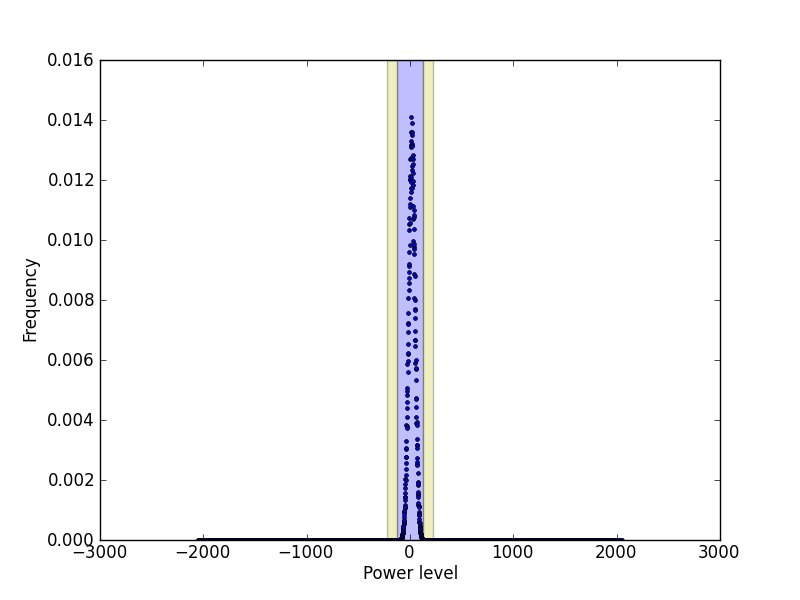
\includegraphics[width=0.5\textwidth]{plots/Stand001Xhist.png}} 				\subfloat{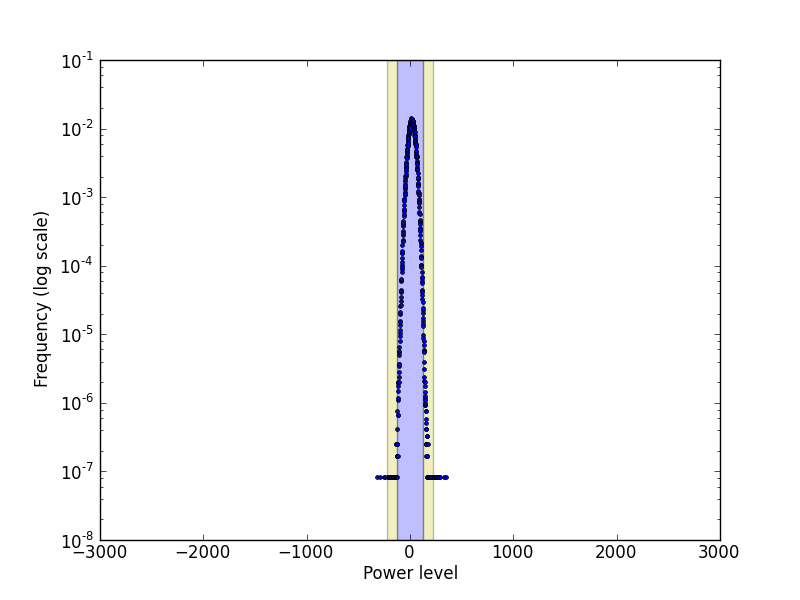
\includegraphics[width=0.5\textwidth]{plots/Stand001Xhist_log.png}} 				\caption{Data from Stand001X. RMS is 34.118799 Samples used : 3792000000. If the RMS is unchanged 99.989642 percent of the samples will lie within [-128,128).  				 With an RMS of 20 99.999833 percent of the samples will lie within [-128,128).} 				\end{figure} 

\begin{figure}[ht] 				\subfloat{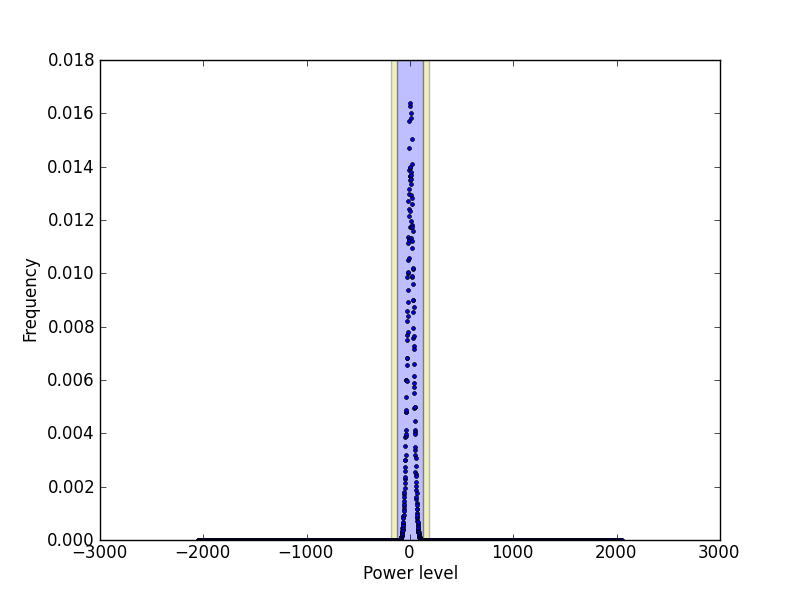
\includegraphics[width=0.5\textwidth]{plots/Stand001Yhist.png}} 				\subfloat{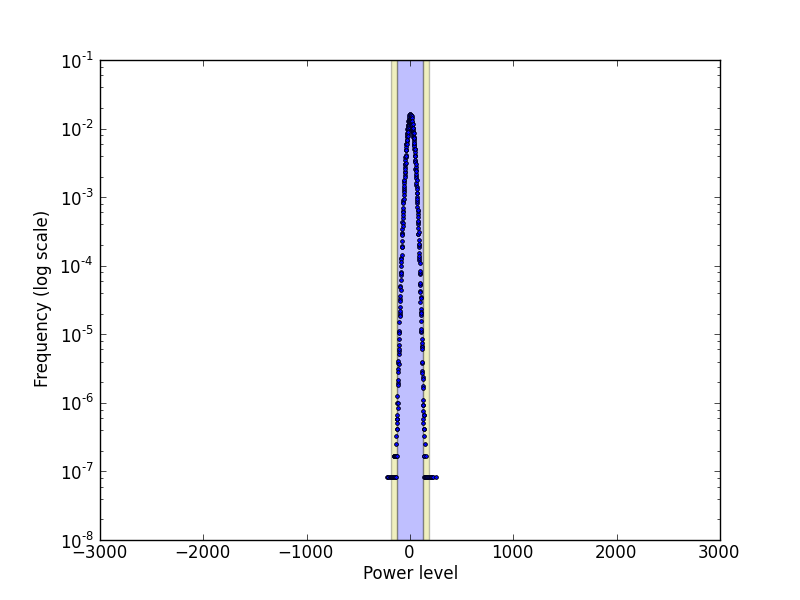
\includegraphics[width=0.5\textwidth]{plots/Stand001Yhist_log.png}} 				\caption{Data from Stand001Y. RMS is 28.544381 Samples used : 3792000000. If the RMS is unchanged 99.998850 percent of the samples will lie within [-128,128).  				 With an RMS of 20 99.999900 percent of the samples will lie within [-128,128).} 				\end{figure} 

\begin{figure}[ht] 				\subfloat{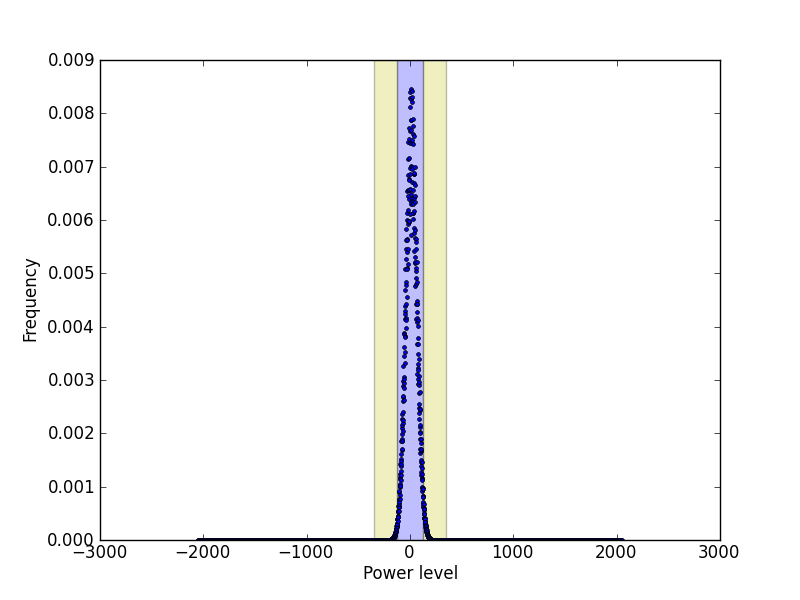
\includegraphics[width=0.5\textwidth]{plots/Stand010Xhist.png}} 				\subfloat{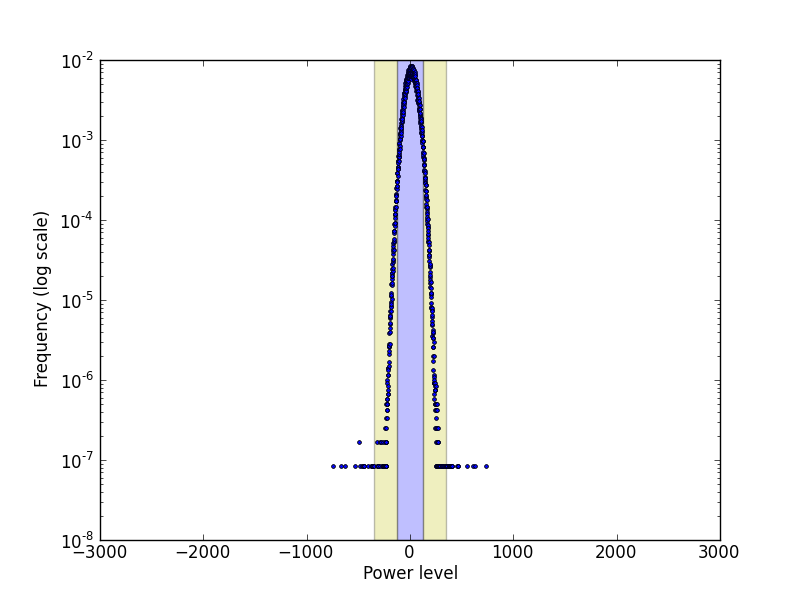
\includegraphics[width=0.5\textwidth]{plots/Stand010Xhist_log.png}} 				\caption{Data from Stand010X. RMS is 55.174325 Samples used : 3792000000. If the RMS is unchanged 98.006408 percent of the samples will lie within [-128,128).  				 With an RMS of 20 99.999708 percent of the samples will lie within [-128,128).} 				\end{figure} 

\begin{figure}[ht] 				\subfloat{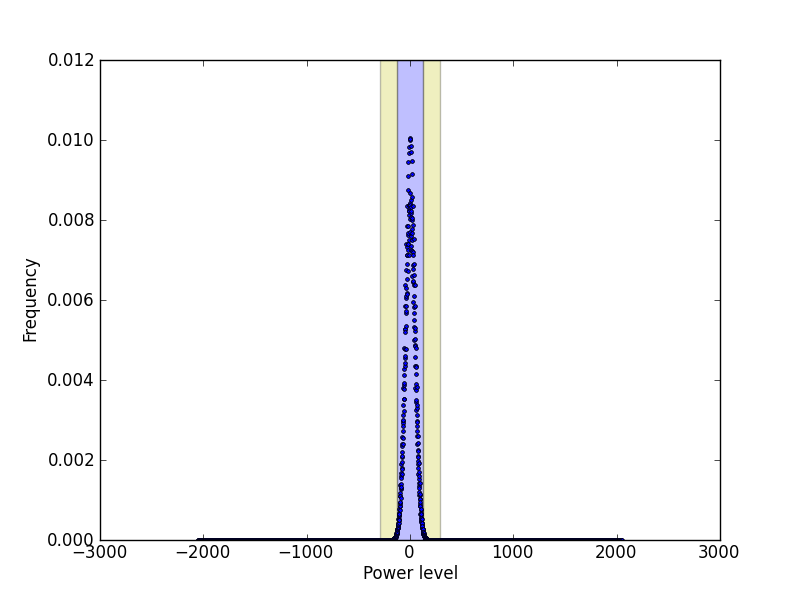
\includegraphics[width=0.5\textwidth]{plots/Stand010Yhist.png}} 				\subfloat{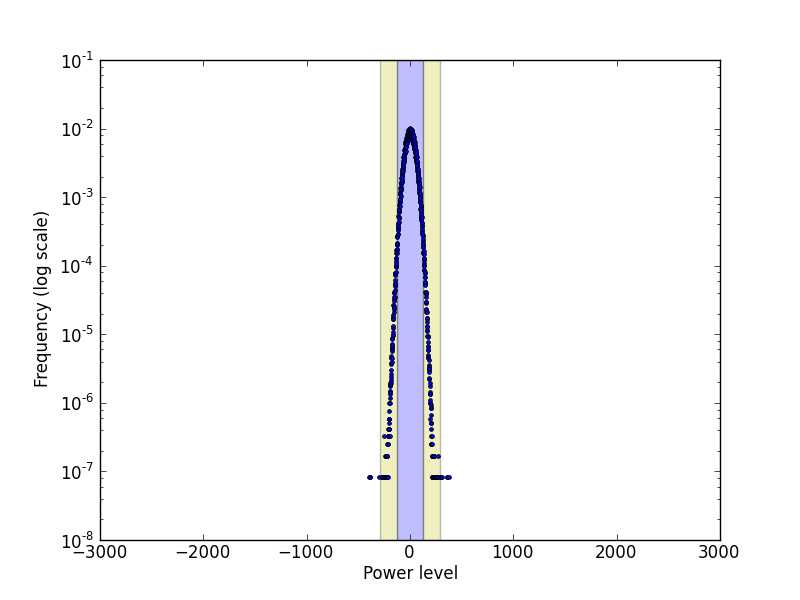
\includegraphics[width=0.5\textwidth]{plots/Stand010Yhist_log.png}} 				\caption{Data from Stand010Y. RMS is 46.112851 Samples used : 3792000000. If the RMS is unchanged 99.452792 percent of the samples will lie within [-128,128).  				 With an RMS of 20 99.999925 percent of the samples will lie within [-128,128).} 				\end{figure} 

\begin{figure}[ht] 				\subfloat{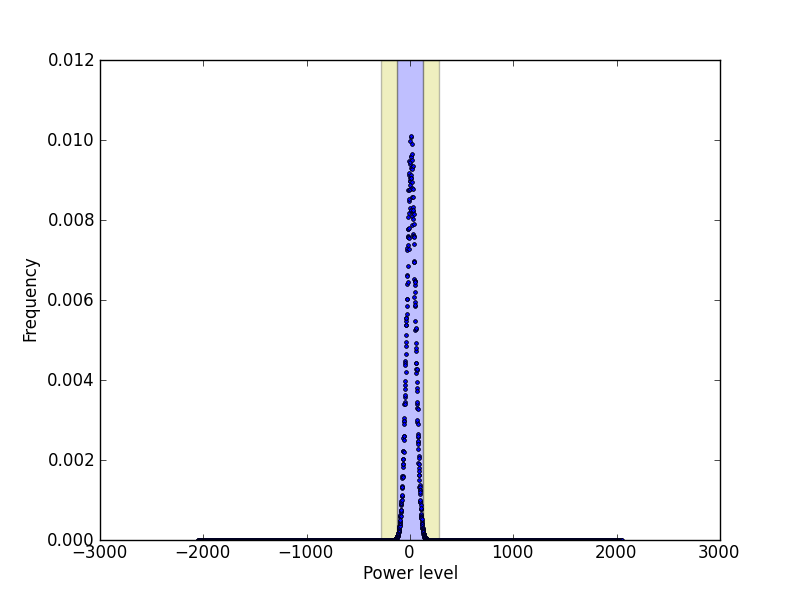
\includegraphics[width=0.5\textwidth]{plots/Stand054Xhist.png}} 				\subfloat{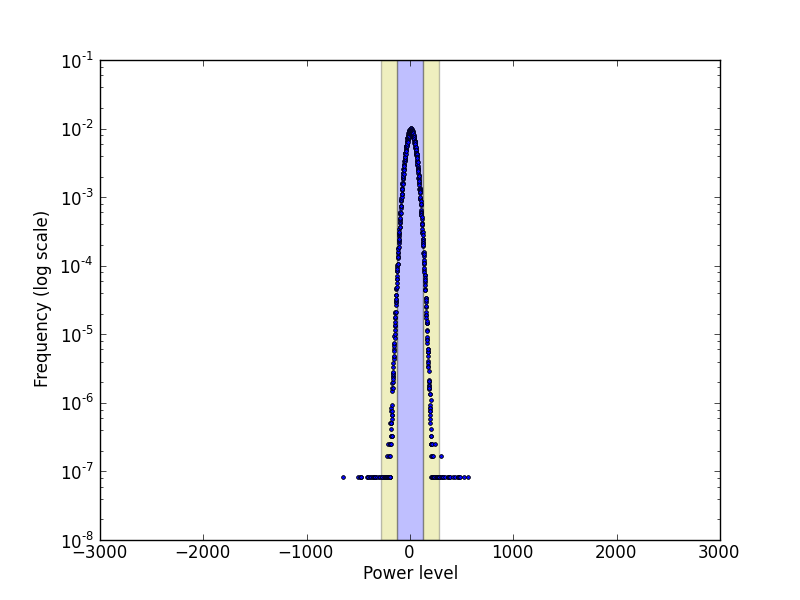
\includegraphics[width=0.5\textwidth]{plots/Stand054Xhist_log.png}} 				\caption{Data from Stand054X. RMS is 43.717739 Samples used : 3792000000. If the RMS is unchanged 99.662692 percent of the samples will lie within [-128,128).  				 With an RMS of 20 99.999642 percent of the samples will lie within [-128,128).} 				\end{figure} 

\begin{figure}[ht] 				\subfloat{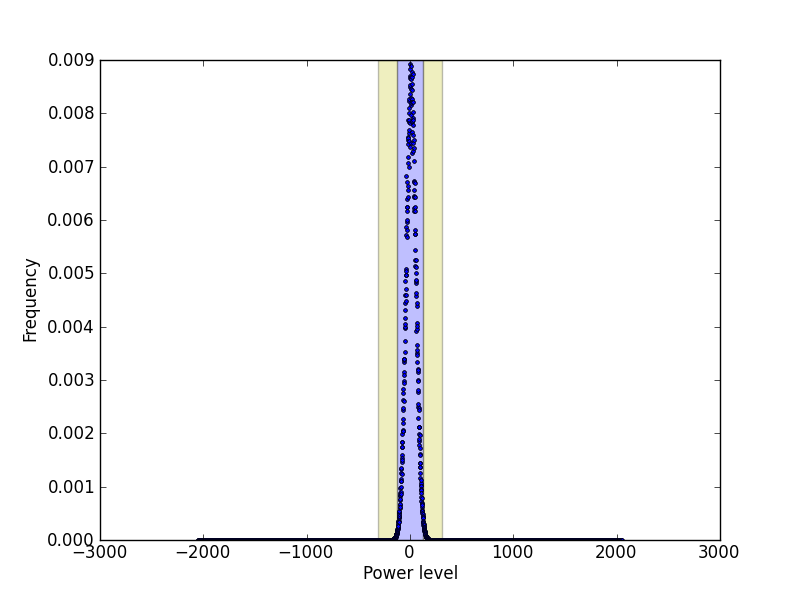
\includegraphics[width=0.5\textwidth]{plots/Stand054Yhist.png}} 				\subfloat{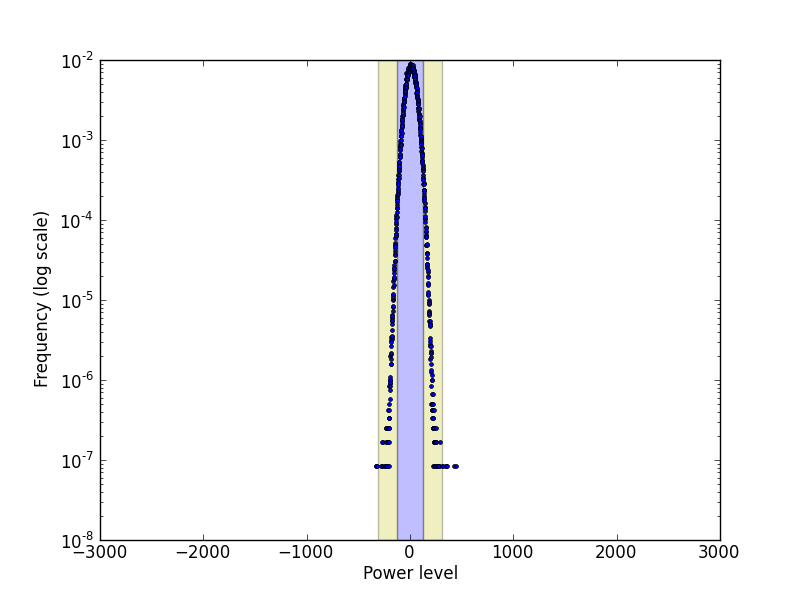
\includegraphics[width=0.5\textwidth]{plots/Stand054Yhist_log.png}} 				\caption{Data from Stand054Y. RMS is 47.889111 Samples used : 3792000000. If the RMS is unchanged 99.243642 percent of the samples will lie within [-128,128).  				 With an RMS of 20 99.999917 percent of the samples will lie within [-128,128).} 				\end{figure} 

\begin{figure}[ht] 				\subfloat{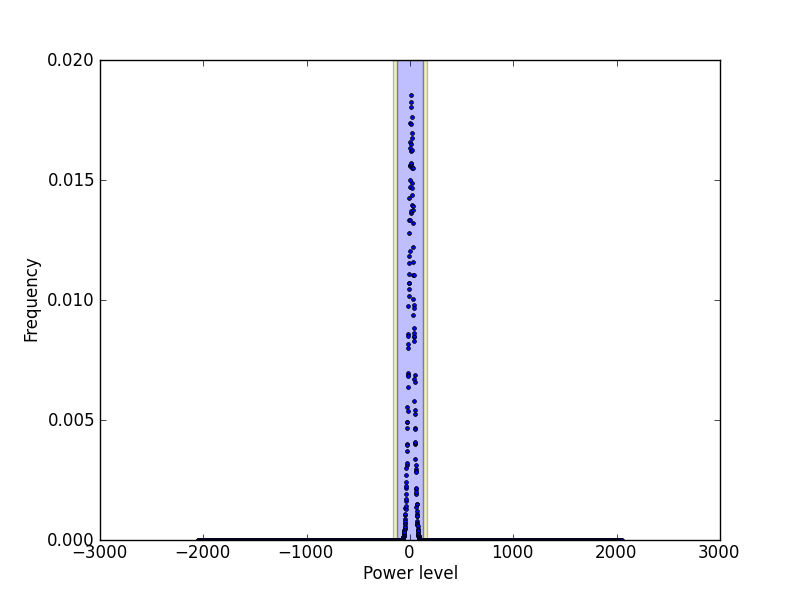
\includegraphics[width=0.5\textwidth]{plots/Stand248Xhist.png}} 				\subfloat{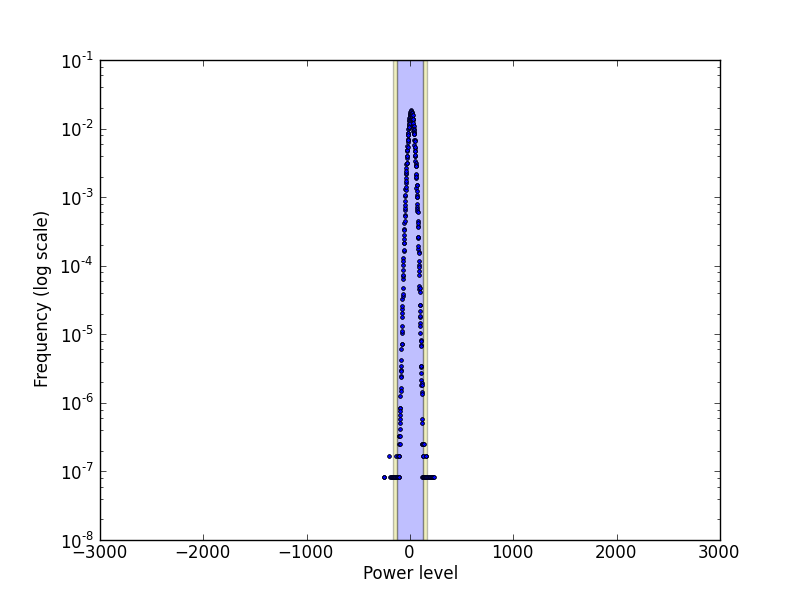
\includegraphics[width=0.5\textwidth]{plots/Stand248Xhist_log.png}} 				\caption{Data from Stand248X. RMS is 26.123760 Samples used : 3792000000. If the RMS is unchanged 99.999583 percent of the samples will lie within [-128,128).  				 With an RMS of 20 99.999850 percent of the samples will lie within [-128,128).} 				\end{figure} 

\begin{figure}[ht] 				\subfloat{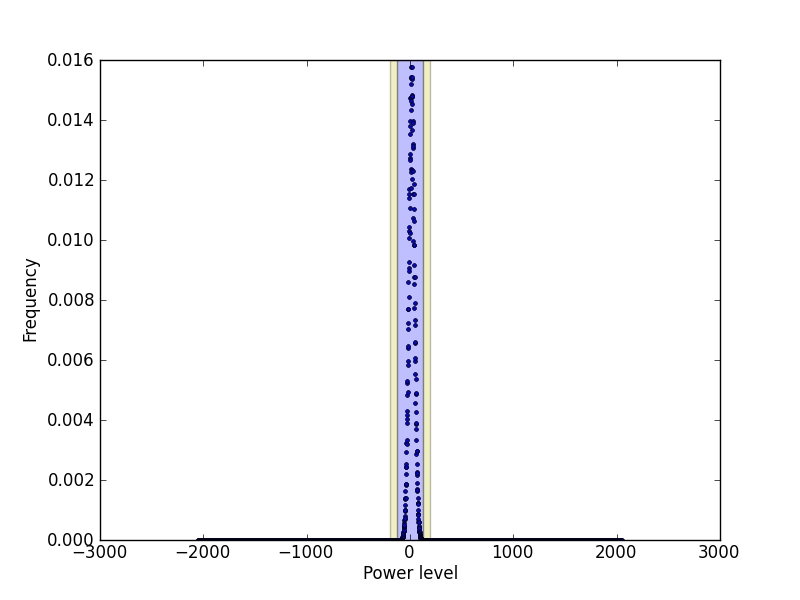
\includegraphics[width=0.5\textwidth]{plots/Stand248Yhist.png}} 				\subfloat{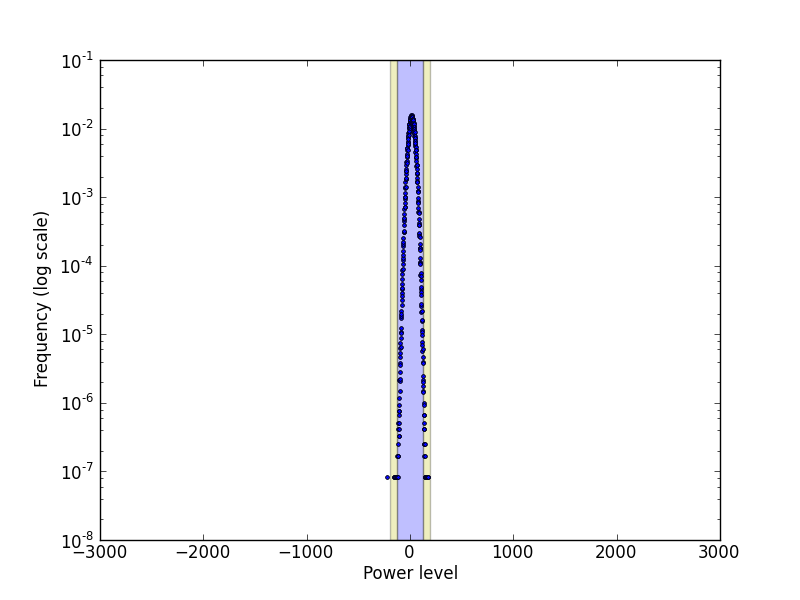
\includegraphics[width=0.5\textwidth]{plots/Stand248Yhist_log.png}} 				\caption{Data from Stand248Y. RMS is 30.707551 Samples used : 3792000000. If the RMS is unchanged 99.998758 percent of the samples will lie within [-128,128).  				 With an RMS of 20 99.999992 percent of the samples will lie within [-128,128).} 				\end{figure} 

\begin{figure}[ht] 				\subfloat{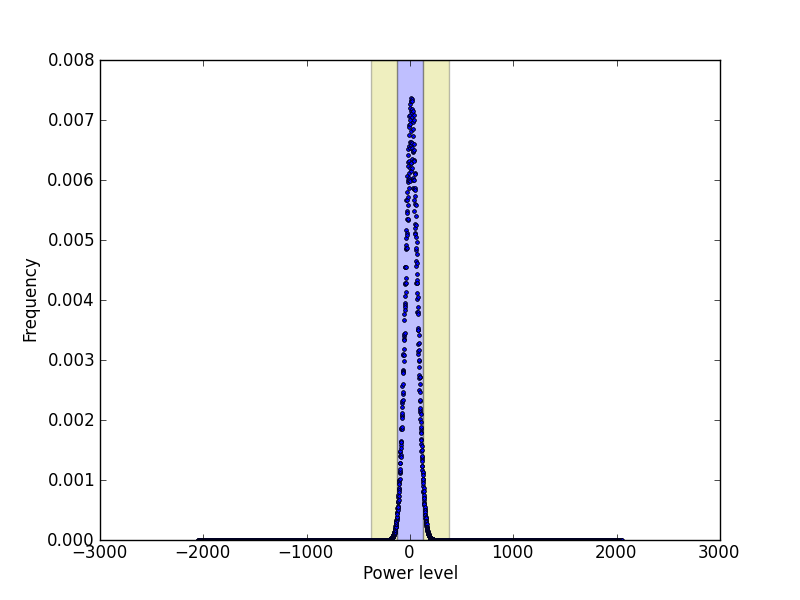
\includegraphics[width=0.5\textwidth]{plots/Stand251Xhist.png}} 				\subfloat{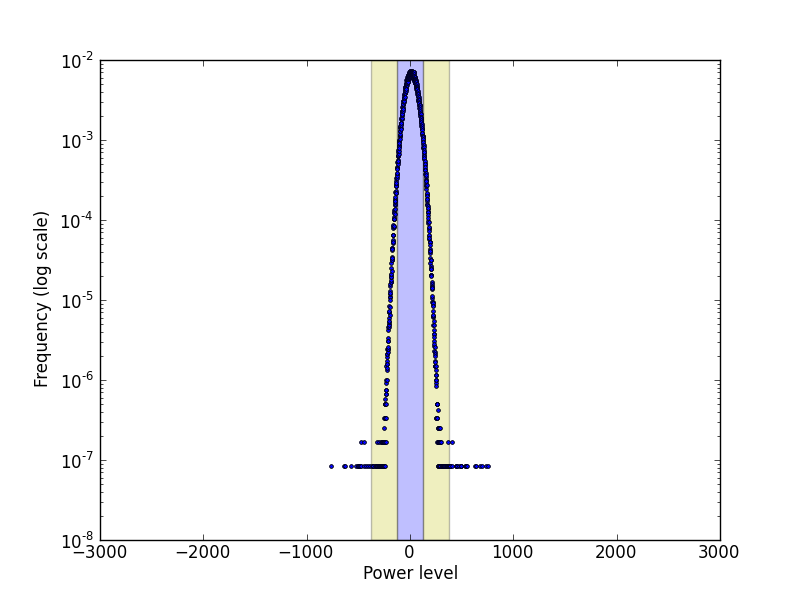
\includegraphics[width=0.5\textwidth]{plots/Stand251Xhist_log.png}} 				\caption{Data from Stand251X. RMS is 58.756399 Samples used : 3792000000. If the RMS is unchanged 97.093867 percent of the samples will lie within [-128,128).  				 With an RMS of 20 99.999633 percent of the samples will lie within [-128,128).} 				\end{figure} 

\begin{figure}[ht] 				\subfloat{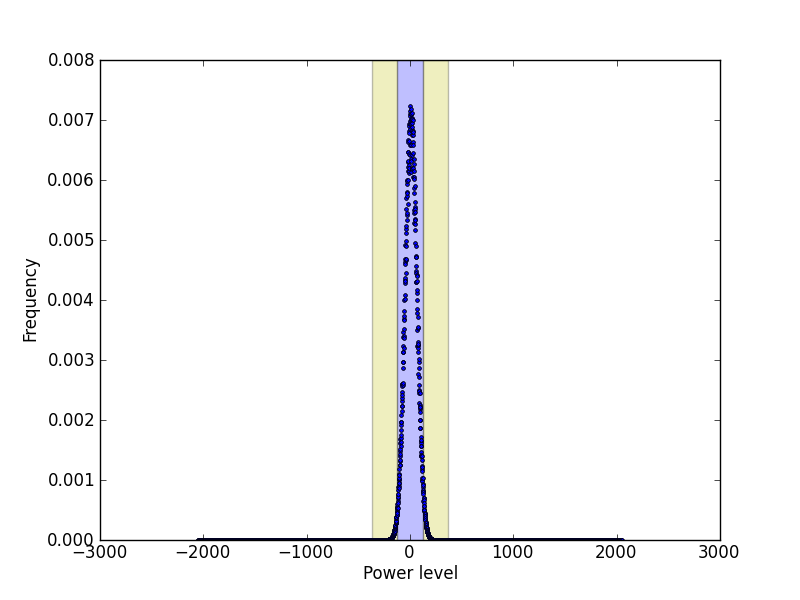
\includegraphics[width=0.5\textwidth]{plots/Stand251Yhist.png}} 				\subfloat{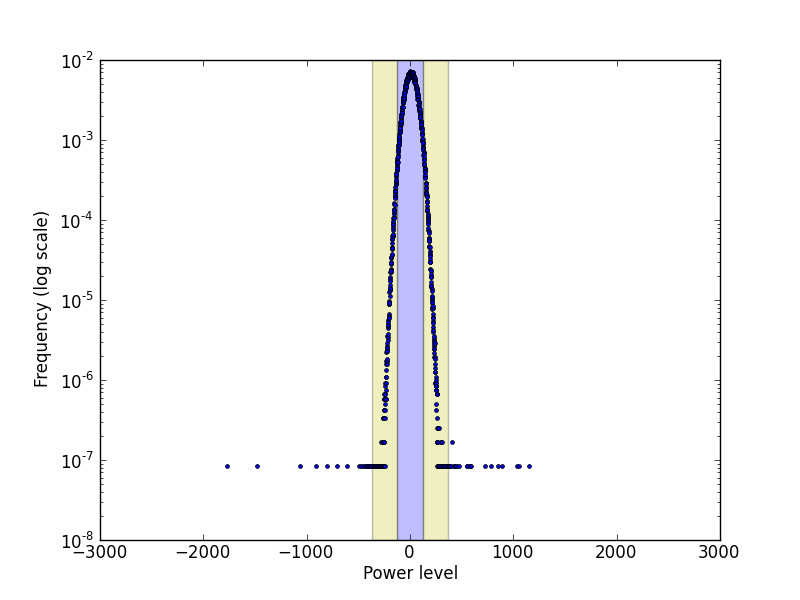
\includegraphics[width=0.5\textwidth]{plots/Stand251Yhist_log.png}} 				\caption{Data from Stand251Y. RMS is 58.047033 Samples used : 3792000000. If the RMS is unchanged 97.285133 percent of the samples will lie within [-128,128).  				 With an RMS of 20 99.999650 percent of the samples will lie within [-128,128).} 				\end{figure} 

\begin{figure}[ht] 				\subfloat{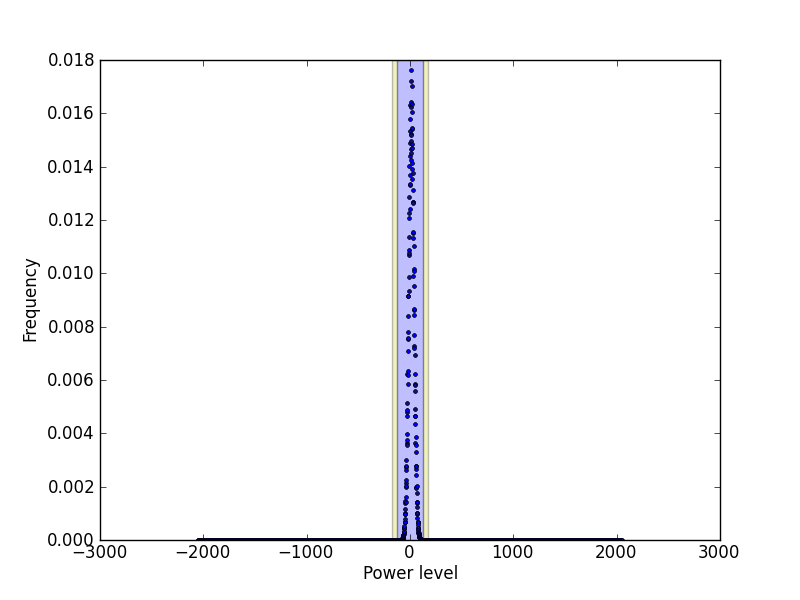
\includegraphics[width=0.5\textwidth]{plots/Stand258Xhist.png}} 				\subfloat{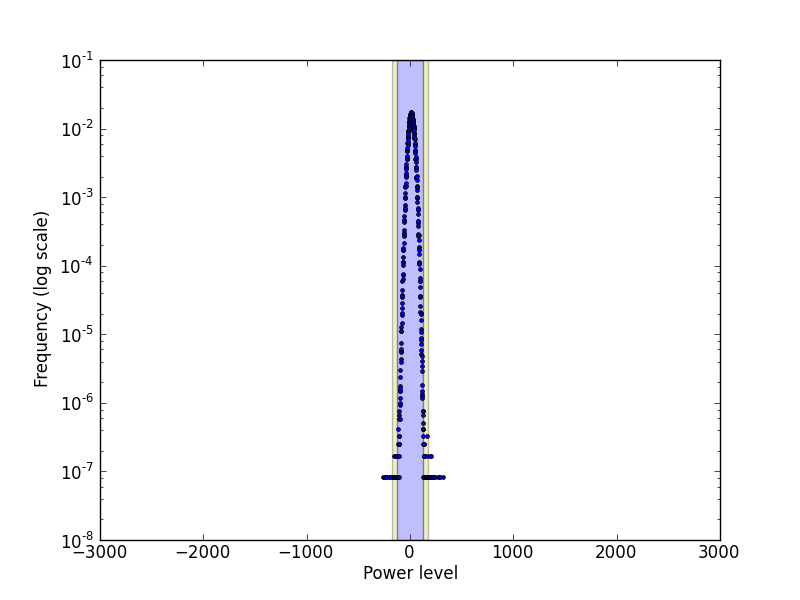
\includegraphics[width=0.5\textwidth]{plots/Stand258Xhist_log.png}} 				\caption{Data from Stand258X. RMS is 27.404131 Samples used : 3792000000. If the RMS is unchanged 99.999292 percent of the samples will lie within [-128,128).  				 With an RMS of 20 99.999767 percent of the samples will lie within [-128,128).} 				\end{figure} 

\begin{figure}[ht] 				\subfloat{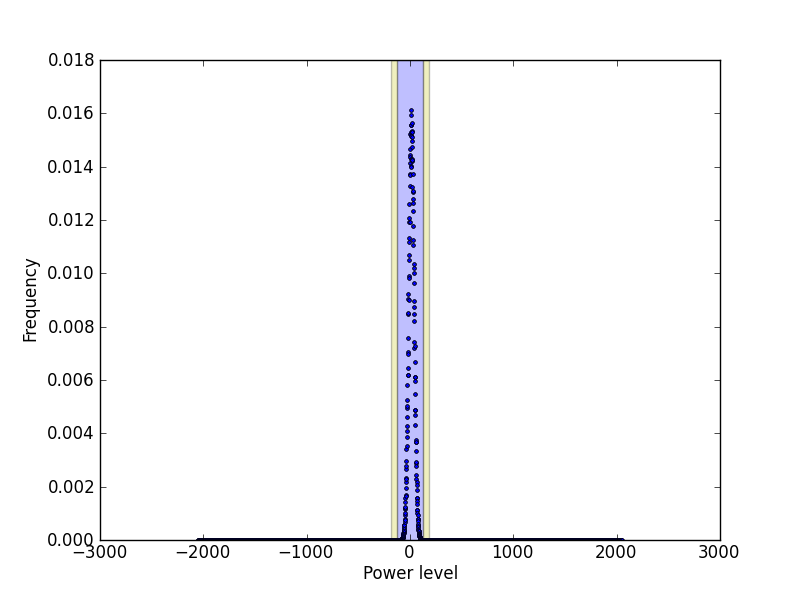
\includegraphics[width=0.5\textwidth]{plots/Stand258Yhist.png}} 				\subfloat{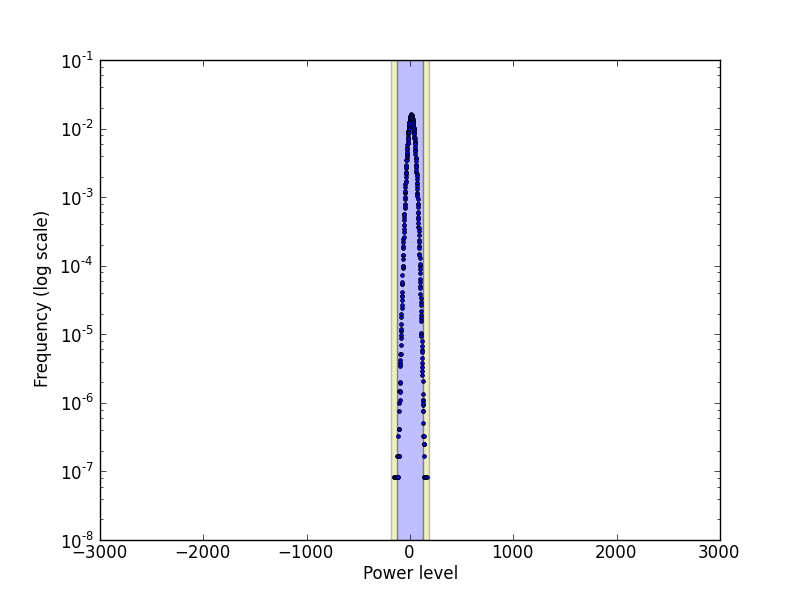
\includegraphics[width=0.5\textwidth]{plots/Stand258Yhist_log.png}} 				\caption{Data from Stand258Y. RMS is 28.380539 Samples used : 3792000000. If the RMS is unchanged 99.999533 percent of the samples will lie within [-128,128).  				 With an RMS of 20 100.000000 percent of the samples will lie within [-128,128).} 				\end{figure} 

